% Group 1 - GAPBS BFS - presentation (20 min + 5 min Q&A), 20/22 October 2026
% Build: pdflatex slides.tex (twice). Figures come from ../report/figures.
\documentclass[aspectratio=169,11pt]{beamer}
\usepackage[T1]{fontenc}
\usepackage[utf8]{inputenc}
\usepackage{lmodern}
\usepackage{booktabs,siunitx,tikz,amsmath}
\usetikzlibrary{arrows.meta,positioning,calc}
\graphicspath{{../report/figures/}{rug/}}
\sisetup{group-separator={,}}

% ---------------------------------------------------------------- RUG-style theme
\definecolor{rugred}{RGB}{204,0,0}
\definecolor{rugdark}{RGB}{88,0,0}
\definecolor{ruggray}{RGB}{60,60,60}
\definecolor{ruglight}{RGB}{150,150,150}
\definecolor{rugpale}{RGB}{250,235,235}
\setbeamertemplate{navigation symbols}{}
\setbeamercolor{normal text}{fg=ruggray}
\setbeamercolor{structure}{fg=rugred}
\setbeamercolor{alerted text}{fg=rugred}
\setbeamercolor{frametitle}{fg=ruggray}
\setbeamerfont{frametitle}{size=\LARGE,series=\bfseries}
\setbeamertemplate{itemize items}[circle]
\setbeamercolor{itemize item}{fg=ruggray}
\setbeamercolor{itemize subitem}{fg=ruglight}
\setbeamertemplate{frametitle}{\vspace*{0.45cm}\insertframetitle\par\vspace*{-0.1cm}}
\setbeamertemplate{headline}{%
  \begin{tikzpicture}[remember picture,overlay]
    \node[anchor=north east,inner sep=0] at ([xshift=-0.35cm,yshift=-0.25cm]current page.north east)
      {
\includegraphics[height=1.0cm]{rug_crest}};
  \end{tikzpicture}}
\setbeamertemplate{footline}{%
  \hspace*{0.5cm}{\tiny\color{ruglight}2026-10-20\quad Group 1: GAPBS BFS}\hfill
  {\tiny\color{ruglight}\insertframenumber/\inserttotalframenumber}\hspace*{0.5cm}\vspace*{0.25cm}}
\setbeamersize{text margin left=0.9cm,text margin right=0.9cm}
\newcommand{\hl}[1]{\textcolor{rugred}{\textbf{#1}}}
\newcommand{\fig}[2][]{\includegraphics[#1]{#2}}

\begin{document}

% ---------------------------------------------------------------- title
{\usebackgroundtemplate{
\includegraphics[width=\paperwidth,height=\paperheight]{title_background}}
\setbeamertemplate{headline}{}\setbeamertemplate{footline}{}
\begin{frame}[plain]
  \vspace*{-0.4cm}
  
\includegraphics[height=1.15cm]{rug_wordmark_red}\par
  \vspace*{1.6cm}
  {\color{white}\fontsize{24}{28}\selectfont\bfseries Performance Engineering of\\[2pt]
   Direction-Optimising BFS (GAPBS)\par}
  \vspace*{0.25cm}
  {\color{white}\large\bfseries WMCS045-05 \textperiodcentered{} Group 1\par}
  \vspace*{1.3cm}
  {\color{white}\bfseries Sergiu Alexandru Macra \quad Cosmin Andrei Stamate\par}
  \vspace*{0.1cm}
  {\color{white}\small Bernoulli Institute \hfill 2026-10-20\par}
\end{frame}}

% ---------------------------------------------------------------- overview
\begin{frame}{Overview}
  \vspace*{0.4cm}
  \begin{enumerate}\setlength{\itemsep}{6pt}\large
    \item Application and systems
    \item Measurement method and tool validation
    \item Performance analysis
    \item Performance model
    \item Optimisations
    \item Conclusions
  \end{enumerate}
\end{frame}

% ---------------------------------------------------------------- application
\begin{frame}{Application: direction-optimising BFS}
  \begin{columns}[T]
    \begin{column}{0.52\textwidth}
      \begin{itemize}\setlength{\itemsep}{4pt}
        \item GAP Benchmark Suite, \texttt{bfs}: CSR graph, OpenMP
        \item \textbf{Top-down} (\texttt{TDStep}): frontier pushes to neighbours,
              random CAS on \texttt{parent[v]}
        \item \textbf{Bottom-up} (\texttt{BUStep}): every unvisited vertex searches its
              neighbours for a frontier vertex and \emph{stops at the first hit}
        \item Switch by $\alpha=15$, $\beta=18$; conversions \texttt{QueueToBitmap},
              \texttt{BitmapToQueue}
        \item Input \texttt{kron20}: $2^{20}$ vertices, 15.7\,M edges, \SI{136}{MB}
      \end{itemize}
    \end{column}
    \begin{column}{0.45\textwidth}
      \centering
      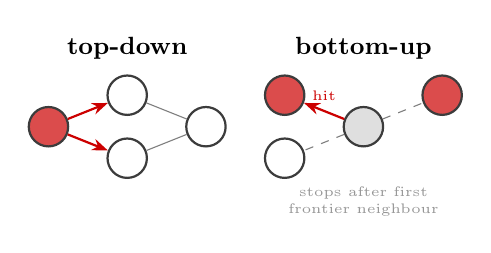
\begin{tikzpicture}[v/.style={circle,draw=ruggray,thick,minimum size=5mm,inner sep=0},
                          f/.style={v,fill=rugred!70},>={Stealth[length=2mm]}]
        \node[font=\small\bfseries] at (1.0,2.2) {top-down};
        \node[f] (a) at (0,1.2) {}; \node[v] (b) at (1.0,1.6) {}; \node[v] (c) at (1.0,0.8) {};
        \node[v] (d) at (2.0,1.2) {};
        \draw[->,thick,rugred] (a) -- (b); \draw[->,thick,rugred] (a) -- (c);
        \draw[gray] (b) -- (d); \draw[gray] (c) -- (d);
        \node[font=\small\bfseries] at (4.0,2.2) {bottom-up};
        \node[f] (e) at (3.0,1.6) {}; \node[v] (g) at (3.0,0.8) {}; \node[v,fill=gray!25] (h) at (4.0,1.2) {};
        \node[f] (i) at (5.0,1.6) {};
        \draw[->,thick,rugred] (h) -- (e) node[midway,above,font=\tiny,text=rugred] {hit};
        \draw[gray,dashed] (h) -- (g); \draw[gray,dashed] (h) -- (i);
        \node[font=\tiny,text=ruglight,align=center] at (4.0,0.25) {stops after first\\ frontier neighbour};
      \end{tikzpicture}
      \vspace*{0.4cm}

      \colorbox{rugpale}{\parbox{0.92\linewidth}{\centering\small
        Edge counters we added: a search examines only\\
        {\Large\hl{4.7\,\%}} of the 31.4\,M directed edges.\\
        TEPS overstates the real work by $\approx20\times$.}}
    \end{column}
  \end{columns}
\end{frame}

% ---------------------------------------------------------------- systems
\begin{frame}{Systems}
  \footnotesize
  \begin{tabular}{@{}p{3.6cm}p{5.2cm}p{5.2cm}@{}}
    \toprule
    & \textbf{Laptop} & \textbf{Hábrók node} \\
    \midrule
    CPU & Intel i7-12650H (6P+4E), WSL2: 10 vCPUs & 2$\times$ AMD EPYC 7763, 128 cores, 2 NUMA \\
    STREAM triad (all / 1 thread) & \SI{15.9}{GB/s} / \SI{12.3}{GB/s} & \SI{327}{GB/s} / \SI{34.7}{GB/s} \\
    DRAM latency (\SI{1}{GB}) & \SI{376}{ns} & \SI{99}{ns} \\
    Measured MLP per core & 15.7 & 21.7 \\
    Counters & \alert{none} (WSL2 hides the PMU) & PAPI 7.1 (built by us), pecount \\
    \bottomrule
  \end{tabular}

  \vspace*{0.5cm}
  \begin{itemize}\setlength{\itemsep}{3pt}
    \item No HAICGU access $\Rightarrow$ Hábrók instead. No perf, PAPI or numactl there:
          we \textbf{built PAPI} and wrote \textbf{pecount} (\texttt{perf\_event\_open}, 200 lines)
    \item Everything runs from one batch script per platform; 30 variants via compile-time switches
  \end{itemize}
\end{frame}

% ---------------------------------------------------------------- method
\begin{frame}{Measurement method}
  \begin{columns}[c]
    \begin{column}{0.5\textwidth}
      \begin{itemize}\setlength{\itemsep}{5pt}
        \item 1 discarded run, then 5 processes $\times$ 24 searches
        \item \textbf{Drop trials 1--5} of each process: warm-up is up to 50$\times$ slower on Hábrók
        \item Report \textbf{median and IQR}; GTEPS $=m/t$
        \item Significant only if the difference exceeds \textbf{both IQRs}
        \item \textbf{Every variant must pass the BFS verifier} before it is timed
      \end{itemize}
    \end{column}
    \begin{column}{0.48\textwidth}
      \centering\fig[width=\linewidth]{warmup}
    \end{column}
  \end{columns}
\end{frame}

% ---------------------------------------------------------------- tool validation
\begin{frame}{Do the tools measure what we think?}
  \small
  \begin{tabular}{@{}lll@{}}
    \toprule
    Check & Result & Verdict \\
    \midrule
    3 wall-clock sources (laptop) & \SIlist{0.679;0.717;0.69}{s} & agree \\
    perf task-clock vs.\ \texttt{time} & \SI{6.00}{s} vs.\ \SI{6.05}{s} & agree \\
    pecount vs.\ perf & page faults \num{36422} vs.\ \num{36423} & agree \\
    PAPI regions vs.\ pecount & misses \SI{99.1}{\percent}, cycles \SI{95}{\percent} & agree \\
    Known answer: ALU chain & \textbf{5.000} instr., \textbf{4.000} cycles / iter. & = \texttt{imul}+\texttt{add} loop \\
    Known answer: \SI{1}{GB} chase & \textbf{1.0007} misses / step & exact \\
    gprof & \SI{100}{\percent} in \texttt{frame\_dummy} & \alert{unusable for OpenMP} \\
    pecount, multiplexed & 2.4 misses / step & \alert{scaling breaks} \\
    \bottomrule
  \end{tabular}
\end{frame}

% ---------------------------------------------------------------- data race
\begin{frame}{Verification found a hidden data race}
  \begin{columns}[c]
    \begin{column}{0.55\textwidth}
      \begin{itemize}\setlength{\itemsep}{5pt}
        \item \texttt{BUStep} sets bits in a shared bitmap \textbf{without atomics}
        \item Safe only if each thread's chunk starts on a 64-bit word
        \item Upstream \texttt{dynamic,1024} satisfies this \emph{by accident}
        \item $\Rightarrow$ schedule sweep restricted to chunk sizes that are multiples of 64
      \end{itemize}
    \end{column}
    \begin{column}{0.4\textwidth}
      \centering\small
      \begin{tabular}{@{}lrr@{}}
        \toprule
        \texttt{OMP\_SCHEDULE} & Laptop & Hábrók \\
        \midrule
        \texttt{dynamic,1024} & 8/8 & 8/8 \\
        \texttt{dynamic,64} & 8/8 & 8/8 \\
        \texttt{static,1000} & \alert{4/8} & \alert{0/8} \\
        \texttt{dynamic,100} & \alert{0/8} & \alert{0/8} \\
        \texttt{guided} & \alert{0/8} & \alert{0/8} \\
        \bottomrule
      \end{tabular}\\[2pt]
      {\scriptsize correct BFS trees out of 8}
    \end{column}
  \end{columns}
\end{frame}

% ---------------------------------------------------------------- hotspots
\begin{frame}{Where does the time go?}
  \begin{columns}[T]
    \begin{column}{0.47\textwidth}
      \textbf{Laptop, perf sampling (10 threads)}\\[3pt]
      \small
      \begin{tabular}{@{}lr@{}}
        \toprule
        OpenMP runtime (barrier spin) & \alert{\SI{50.0}{\percent}} \\
        \texttt{BUStep} & \SI{35.8}{\percent} \\
        \texttt{InitParent} & \SI{5.7}{\percent} \\
        \texttt{TDStep} & \SI{3.1}{\percent} \\
        conversions + rest & \SI{5.4}{\percent} \\
        \bottomrule
      \end{tabular}\\[4pt]
      \footnotesize \SI{39}{\percent} of \texttt{BUStep} samples on the miss to the start of a
      neighbour list
    \end{column}
    \begin{column}{0.5\textwidth}
      \textbf{Hábrók, PAPI per kernel (1 thread)}\\[3pt]
      \small
      \begin{tabular}{@{}lrrr@{}}
        \toprule
        Kernel & Cycles & IPC & Misses \\
        \midrule
        \texttt{BUStep} & \SI{78}{\percent} & 0.77 & 0.32 / vertex \\
        \texttt{InitParent} & \SI{14}{\percent} & 0.89 & -- \\
        \texttt{TDStep} & \SI{4}{\percent} & 1.01 & 0.75 / edge \\
        conversions & \SI{4}{\percent} & 1.6--4.8 & -- \\
        \bottomrule
      \end{tabular}\\[4pt]
      \footnotesize memory-bound: low IPC; TLB irrelevant with THP (4.2k misses / search)
    \end{column}
  \end{columns}
\end{frame}

% ---------------------------------------------------------------- scaling
\begin{frame}{Thread scaling}
  \centering\fig[width=0.92\linewidth]{scaling}
  \begin{itemize}\small
    \item Laptop: flat beyond 8 threads. Hábrók: best at \hl{48--64 bound threads} (one
          socket), \alert{slower again at 128}
    \item The server has 13$\times$ the cores and 20$\times$ the bandwidth, but is only 3$\times$ faster. Why?
  \end{itemize}
\end{frame}

% ---------------------------------------------------------------- model
\begin{frame}{Model: bytes and random accesses, not FLOPs}
  \begin{columns}[T]
    \begin{column}{0.5\textwidth}
      \small
      \begin{itemize}\setlength{\itemsep}{3pt}
        \item Roofline in FLOP/byte: BFS has no FLOPs
        \item ECM: needs predictable steady-state loops
        \item $\Rightarrow$ \textbf{information-exchange model} from measured work
      \end{itemize}
      \vspace*{-0.1cm}
      \begin{align*}
        T_\text{bw}(p) &= \frac{Q}{\min(p B_1, B_\text{all})}\\
        T_\text{lat}(p) &= \frac{N_\text{rand}\,L_\text{DRAM}}{\text{MLP}\cdot p}
      \end{align*}
      \footnotesize All parameters measured: edge counters, STREAM, pointer chase, MLP benchmark
    \end{column}
    \begin{column}{0.47\textwidth}
      \small
      \begin{tabular}{@{}lr@{}}
        \toprule
        Traffic per \texttt{kron20} search & MB \\
        \midrule
        \texttt{InitParent} & 12.6 \\
        bottom-up sweeps & 31.8 \\
        bottom-up neighbour lines & \textbf{106.2} \\
        top-down edges + \texttt{parent[v]} & 19.5 \\
        conversions, final pass & 8.7 \\
        \midrule
        $Q$ & \textbf{178.8} \\
        $N_\text{rand}$ & 1.95\,M \\
        \bottomrule
      \end{tabular}
    \end{column}
  \end{columns}
\end{frame}

\begin{frame}{Model vs.\ measurement: three regimes}
  \begin{columns}[c]
    \begin{column}{0.6\textwidth}
      \hspace*{-0.4cm}\fig[width=1.08\linewidth]{model}
    \end{column}
    \begin{column}{0.38\textwidth}
      \small
      \begin{enumerate}\setlength{\itemsep}{5pt}
        \item \textbf{1 thread: latency-bound}\\ laptop within \SI{21}{\percent};
              Hábrók keeps only $\approx$8 of 22 possible misses (MSHRs) in flight
        \item \textbf{Laptop, all threads: bandwidth-bound}\\ 8.4\,ms vs.\ 11.3\,ms DRAM bound
              (L3 reuse) $\Rightarrow$ no headroom
        \item \textbf{Hábrók: neither}\\ 2.5--6.5$\times$ above both bounds:
              \hl{barriers, imbalance, cross-socket traffic}
      \end{enumerate}
    \end{column}
  \end{columns}
\end{frame}

% ---------------------------------------------------------------- optimisations
\begin{frame}{Seven optimisations, judged by IQR}
  \centering\fig[width=0.8\linewidth]{optimisations}\\[-2pt]
  \small
  \begin{tabular}{@{}ll@{}}
    \hl{Significant:} & relabelling, thread count \& placement, NUMA first touch \\
    \textcolor{ruglight}{\textbf{Within noise:}} & compiler flags, schedules, huge pages, prefetch, $\alpha/\beta$ \\
  \end{tabular}
\end{frame}

\begin{frame}{O5: degree relabelling (up to 2.8$\times$)}
  \begin{columns}[c]
    \begin{column}{0.5\textwidth}
      \small
      \begin{itemize}\setlength{\itemsep}{4pt}
        \item \textbf{Why:} the model says bottom-up neighbour lines dominate $Q$
        \item Renumber by decreasing degree: hubs get small, adjacent IDs and come
              \emph{first} in every sorted neighbour list
        \item Bottom-up hits a frontier vertex sooner:\\
              \hl{$-35\,\%$} edges examined (kron20), \hl{$-48\,\%$} (kron22)
        \item Laptop 8.58 $\to$ \textbf{3.53\,ms} (2.4$\times$); kron22: 2.8$\times$ laptop,
              1.8$\times$ Hábrók
        \item Caveat: \SI{0.46}{s} one-off cost, amortised after $\approx$90 searches
      \end{itemize}
    \end{column}
    \begin{column}{0.47\textwidth}
      \centering\fig[width=\linewidth]{big_graphs}
    \end{column}
  \end{columns}
\end{frame}

\begin{frame}{O2 + O6: fewer threads, better placement}
  \begin{columns}[T]
    \begin{column}{0.48\textwidth}
      \textbf{O2: thread count and binding}\\[4pt]
      \small
      \begin{itemize}\setlength{\itemsep}{3pt}
        \item No OpenMP schedule beats upstream
        \item 48 threads bound to one socket:\\ 2.85 $\to$ \hl{1.38\,ms (2.1$\times$)}
        \item Smaller barriers and no cross-socket coherence
      \end{itemize}
    \end{column}
    \begin{column}{0.48\textwidth}
      \textbf{O6: NUMA-aware first touch}\\[4pt]
      \small
      \begin{itemize}\setlength{\itemsep}{3pt}
        \item \texttt{read()} puts all \SI{125}{MB} of edges on \emph{one} socket
        \item Parallel zeroing before the read spreads pages
        \item Spread threads: 4.00 $\to$ \hl{1.94\,ms (2.1$\times$)}; kron22: $-11\,\%$
        \item No \texttt{numactl} on Hábrók $\Rightarrow$ fixed in code
      \end{itemize}
    \end{column}
  \end{columns}
\end{frame}

\begin{frame}{What did \emph{not} help, and why}
  \small
  \begin{tabular}{@{}p{3.6cm}p{3.7cm}p{6.4cm}@{}}
    \toprule
    Strategy & Result & Explanation \\
    \midrule
    O1 compiler flags & within IQR & no hot loop vectorises: early \texttt{break}, CAS
      \emph{clobbers memory}; memory-bound anyway \\
    O3 huge pages & within IQR & Hábrók already uses THP \texttt{always}; WSL2 variance hides it \\
    O4 prefetch in top-down & $-11\,\%$ at best, n.s. & top-down is only \SI{3}{\percent} of samples
      (Amdahl) \\
    O7 $\alpha/\beta$ sweep & defaults near-optimal & $\alpha=5$: stays top-down too long, 4.4$\times$ slower \\
    \bottomrule
  \end{tabular}

  \vspace*{0.5cm}
  \centering
  \colorbox{rugpale}{\parbox{0.85\linewidth}{\centering
    The analysis and the model predicted these outcomes \emph{before} we implemented them.}}
\end{frame}

% ---------------------------------------------------------------- conclusion
\begin{frame}{Conclusions}
  \begin{itemize}\setlength{\itemsep}{6pt}
    \item BFS is about \textbf{memory and synchronisation}, not arithmetic: IPC $\approx$ 1,
          4.7\,\% of edges touched
    \item 1 core: latency-bound \textperiodcentered{} laptop: bandwidth-bound \textperiodcentered{}
          128-core node: \hl{barrier- and NUMA-bound}
    \item Validated toolchain: perf, PAPI, pecount, timers; gprof fails on OpenMP;
          verification exposed a data race
    \item Best gains: \hl{relabelling (2.8$\times$)}, \hl{socket-local threads (2.1$\times$)},
          \hl{NUMA first touch (2.1$\times$)}
    \item Next: fuse a level's parallel regions to cut barriers; native-Linux laptop counters
  \end{itemize}
  \vspace*{0.3cm}
  {\footnotesize\color{ruglight} Code, scripts, raw data: \texttt{github.com/CosminStamateAndrei/gapbs} (\texttt{pe/})}
\end{frame}

% ---------------------------------------------------------------- questions
{\setbeamertemplate{headline}{}
\begin{frame}
  \vspace*{0.6cm}
  \begin{columns}[c]
    \begin{column}{0.55\textwidth}
      {\fontsize{30}{34}\selectfont\color{ruggray} Questions?}
    \end{column}
    \begin{column}{0.4\textwidth}
      \centering
\includegraphics[width=0.75\linewidth]{rug_crest}
    \end{column}
  \end{columns}
\end{frame}}

\end{document}
